\chapter{Dealing with extreme low-density chains}
\label{low-density}

\section{Introduction}

As we saw in \cref{genesis}, chain density is our principal means for
distinguishing chains forged by malicious nodes from the honest chain: due to
the fundamental assumption that there is an honest majority, the chain forged by
the honest nodes will be denser than any chain forged by an adversary. If
therefore the honest nodes in the system stop producing blocks due to some
network-wide problem---pervasive node misconfiguration, bug in the ledger,
etc.---the security of the system is at risk. Even when the nodes start
producing blocks again, the low-density region of the chain left behind by the
problem will remain to be an issue for security. If an adversary forks off
their own chain at the point where the honest majority stopped producing blocks,
then new nodes joining the network (using the genesis rule, \cref{genesis}) will
adopt the adversarial chain instead of the honest chain:
%
\begin{center}
\begin{tikzpicture}
\draw
     (0,0)
  -- (3,0) node{$\bullet$} coordinate(i);
\draw
     (i)
  -- ++(3,0) node[pos=0.5,above]{$\overbrace{\hspace{3cm}}^\text{no blocks produced}$}
  -- ++(4,0) node[pos=0.5,above]{$\overbrace{\hspace{4cm}}^\text{chain resumes}$}
             node[right]{honest chain};
\draw
     (i)
  -- ++(0, -1)
  -- ++(4, 0) node[pos=0.5,below]{$\underbrace{\hspace{4cm}}_\text{$s$ slots}$}
  -- ++(2, 0) node[right]{adversarial chain};
\draw [dashed] (7,-2) -- (7,1);
\end{tikzpicture}
\end{center}
%
The \emph{Disaster Recovery Plan}\footnote{Currently not available as a public
document.} sketches how we might ``patch the chain back up'' when a major
problem like this occurs. This must happen out-of-band with the cooperation of
the major stake holders, and is (mostly) outside the scope of the Consensus
Layer report. That said, the options for disaster recovery are currently limited
due to a technical limitation in the consensus layer, which we will discuss now.

From a chain security point of view, it makes little difference if the honest
chain has a region of $s$ slots containing \emph{one} block or \emph{zero}
blocks; both are equally terrible. However, this makes a big
difference to the implementation as it currently stands: as long as there is at
least one block in every $s$ slots, the system can continue; but when there is a
gap of more than $s$ slots anywhere on the chain, the system will grind to a
halt. As we will see in this chapter, this is a consequence of the fact that we
validate headers independent from blocks, the so-called header/body split
(see also \cref{nonfunctional:network:headerbody}). The main goal of this
chapter is to discuss how we can address this, allowing the system to continue
irrespective of any gaps on the chain. This is important for a number of
reasons:

\begin{enumerate}
\item It makes disaster recovery less immediately urgent: if the honest nodes
stop producing blocks for whatever reason, the problem can be resolved, the
system restarted, and blocks can be produced again. Disaster recovery,
and patching the chain back up, can then be considered as the system is running
again, and put into motion when the various stake holders are ready.
\item It also opens up more avenues for disaster recovery. If the consensus
layer can't skip past large gaps on the chain, then the chain \emph{must} be
patched. However, if we lift this restriction, then there are other ways in
which we might address the problem. For example, we could (even if just
temporarily) simply record the low-density area of the chain within the code
itself and hardcode a preference for (this part of the) ``honest but sparse''
chain in chain selection.
\item Chain regions with extreme low density are difficult to avoid
in our consensus tests (\cref{testing:consensus}).
\end{enumerate}

Even \emph{if} it is desirable that the system stops when the chain density
falls below a certain threshold, it does not make sense to set that threshold at
the ``less than 1 block per $s$ slots'' boundary. This should be defined and
implemented as an external policy, not dictated by implementation details.
Moreover, even with an explicit stop, we might like the ability to mark the
known-to-be-low-density chain and restart the system (point 2, above). It is
also far from clear how to avoid adversarial nodes from taking advantage of such
``automatic'' stops (how do we prevent adversaries from producing blocks?).
Either way, such concerns are well outside the scope of this chapter. Here we
address just one question: how can we allow the system to continue when there
are larger-than-$s$-slots gaps on the chain.

\section{Background}

\subsection{Recap: ledger state, ledger view and forecasting}

Blocks are validated against the state of the ledger
(\cref{ledger:api:ApplyBlock}). For example, we check that inputs spent by
transactions in the block are available in the UTxO in the ledger state.
Depending on the choice of consensus protocol, we may also need part of the
ledger state to be able to validate the block \emph{header}. For example, in
Praos and Genesis we need to know the active stake distribution in order to be
able to verify that whoever produced the block had a right to do so. We call the
part of the ledger state that we need to validate block headers the \emph{ledger
view} (\cref{consensus:class:ledgerview}).

We call it a ledger \emph{view} because it is a projection out of the full
ledger state. Unfortunately, we cannot compute the \emph{next} ledger view based only
on the header; there is nothing that corresponds to the dotted arrow in this
diagram:
%
\begin{center}
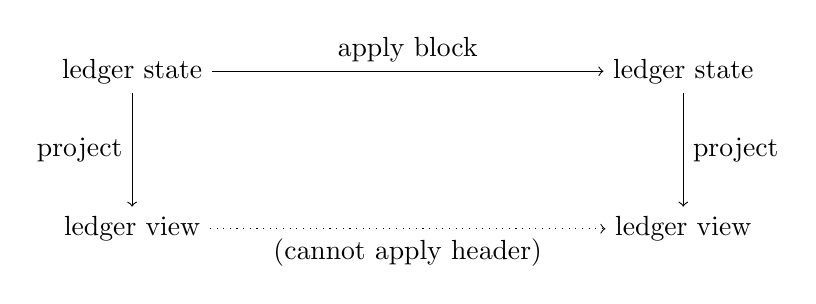
\begin{tikzpicture}[block/.style={rectangle}]
\node at (0, 2) (state1) [block] {ledger state};
\node at (7, 2) (state2) [block] {ledger state};
\node at (0, 0) (view1)  [block] {ledger view};
\node at (7, 0) (view2)  [block] {ledger view};
\draw [->] (state1.south) -- (view1.north) node[pos=0.5,left]{project};
\draw [->] (state2.south) -- (view2.north) node[pos=0.5,right]{project};
\draw [->] (state1.east)  -- (state2.west) node[pos=0.5,above]{apply block};
\draw [->, dotted] (view1.east)  -- (view2.west) node[pos=0.5,below]{(cannot apply header)};
\end{tikzpicture}
\end{center}
%
Let's recall the Praos example again: we can compute the active stake
distribution from the ledger state, but in order to understand how the active
stake distribution evolves, we need to know how the full UTxO evolves, and for
that we need the full blocks. (We discussed this also in
\cref{hfc:failed:forecasting}.)

Let's stay with Praos a little longer. The active stake distribution changes
only at epoch boundaries. Therefore we will know the active stake distribution
at least until the end of the epoch.  Moreover, once we get close enough to the
epoch boundary, we also know the stake distribution for the \emph{next} epoch.
The range over which we know the active stake distribution therefore evolves as
follows:
%
\begin{center}
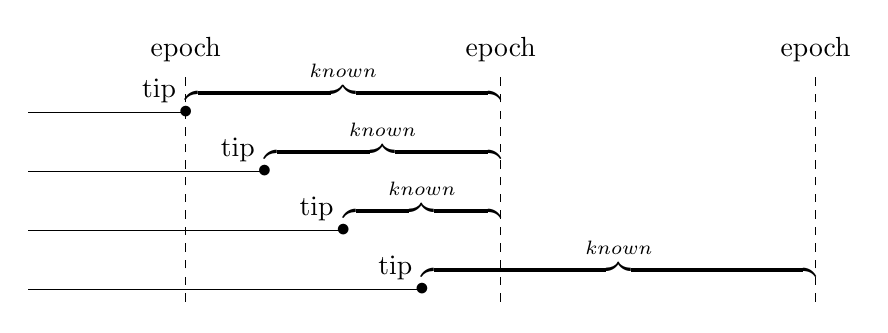
\begin{tikzpicture}[yscale=0.75]
%
\draw (0,  0) -- (2,  0) node{$\bullet$} node[above left]{tip};
\path (2,  0) -- (6,  0) node[pos=0.5,above]{$\overbrace{\hspace{4cm}}^\text{known}$};
%
\draw (0, -1) -- (3, -1) node{$\bullet$} node[above left]{tip};
\path (3, -1) -- (6, -1) node[pos=0.5,above]{$\overbrace{\hspace{3cm}}^\text{known}$};
%
\draw (0, -2) -- (4, -2) node{$\bullet$} node[above left]{tip};
\path (4, -2) -- (6, -2) node[pos=0.5,above]{$\overbrace{\hspace{2cm}}^\text{known}$};
%
\draw (0, -3) -- (5, -3) node{$\bullet$} node[above left]{tip};
\path (9, -3) -- (6, -3) node[pos=0.5,above]{$\overbrace{\hspace{5cm}}^\text{known}$};
%
\draw [dashed] ( 2, -3.2) -- ( 2, 0.7) node[above]{epoch};
\draw [dashed] ( 6, -3.2) -- ( 6, 0.7) node[above]{epoch};
\draw [dashed] (10, -3.2) -- (10, 0.7) node[above]{epoch};
\end{tikzpicture}
\end{center}

\pagebreak

The range over which we know the active stake distribution shrinks and then
grows again, but never falls below a certain minimum size. We abstract from this
process in the consensus layer, and say we can \emph{forecast} the ledger view
from a particular ledger state over a certain \emph{forecast range}
(\cref{ledger:api:LedgerSupportsProtocol}). This does not necessarily mean the
ledger view is constant during that range, but merely that any changes are
\emph{known} (for example, see the last line in the diagram above).

If we change our perspective slightly, we can say that blocks on the chain
cannot influence the ledger view (active stake distribution) until a certain
period of time (in slots) has passed. We call this the \emph{stability window}
of the ledger, and will study it in more detail in the next section.

\subsection{Recap: stability windows}
\label{low-density:recap-stability-window}

Blocks are validated against ledger states; each block is validated against the
ledger state as it was after applying the previous block. This means that when
we validate block $B$ in the example below, we use the ledger state after
applying block $A$; for block $C$, we use the ledger state after applying block
$B$:
%
\begin{center}
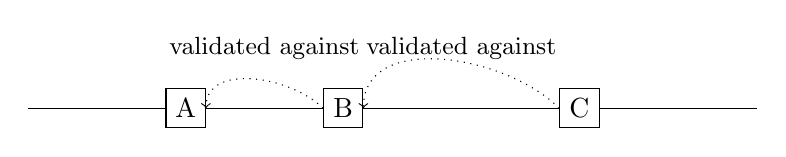
\begin{tikzpicture}
  [block/.style={rectangle,draw=black,minimum size=5mm}
  ,baseline=0pt]
\node at (0,0) (A) [block] {A};
\node at (2,0) (B) [block] {B};
\node at (5,0) (C) [block] {C};
\draw (-2,0)   -- (A.west);
\draw (A.east) -- (B.west) node[pos=0.5,above=5mm]{\small validated against};
\draw (B.east) -- (C.west) node[pos=0.5,above=5mm]{\small validated against};
\draw (C.east) -- ++(2,0);
%
\draw [->, dotted] (B.west) to [out=135,in=90] (A.east);
\draw [->, dotted] (C.west) to [out=135,in=90] (B.east);
\end{tikzpicture}
\qquad
\begin{minipage}{0.25\textwidth}
\emph{Horizontal axis represents time (in slots)}
\end{minipage}
\end{center}
%
In the chain sync client (\cref{chainsyncclient}) we are however not validating
blocks, but block \emph{headers}. As we saw, in order to validate a header we
only need part of the ledger state, known as the ledger \emph{view}. We also saw
that  despite the fact that we only need part of the ledger state, we cannot
\emph{update} the ledger view using only headers: we still need the full block.
This means that if we have block $A$, but only block \emph{headers} $B$ and $C$,
we have a problem:
%
\begin{center}
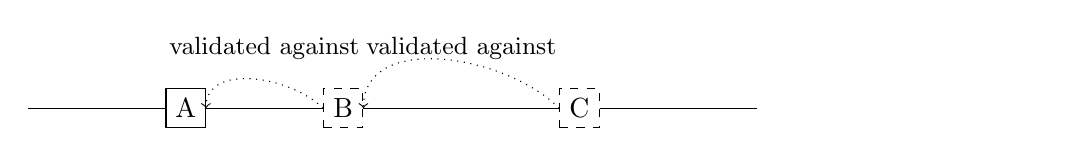
\begin{tikzpicture}
  [block/.style={rectangle,draw=black,minimum size=5mm}]
\path (-2,0) -- (11,0); % adjust bounding box
\node at (0,0) (A) [block] {A};
\node at (2,0) (B) [block, dashed] {B};
\node at (5,0) (C) [block, dashed] {C};
\draw (-2,0)   -- (A.west);
\draw (A.east) -- (B.west) node[pos=0.5,above=5mm]{\small validated against};
\draw (B.east) -- (C.west) node[pos=0.5,above=5mm]{\small validated against};
\draw (C.east) -- ++(2,0);
%
\draw [->, dotted] (B.west) to [out=135,in=90] (A.east);
\draw [->, dotted] (C.west) to [out=135,in=90] (B.east);
\end{tikzpicture}
\end{center}
%
Validating header $B$ is unproblematic, since we have the ledger state available
after applying block $A$. However, since we don't have block $B$, we can't
compute the ledger state after block $B$ to validate header $C$. We are saved by
the fact that we can \emph{forecast} the ledger view  required to validate
header $B$ from the ledger state after $A$:
%
\begin{center}
\begin{tikzpicture}
  [block/.style={rectangle,draw=black,minimum size=5mm}]
\path (-2,0) -- (11,0); % adjust bounding box
\node at (0,0) (A) [block] {A};
\node at (2,0) (B) [block, dashed] {B};
\node at (5,0) (C) [block, dashed] {C};
\draw (-2,0)   -- (A.west);
\draw (A.east) -- (B.west) node[pos=0.55,below=5mm]{\small forecast};
\draw (B.east) -- (C.west);
\draw (C.east) -- ++(2,0);
%
\draw [->, dotted] (B.west) to [out=135,in=90] (A.east);
\draw [->, dotted] (C.west) to [out=135,in=90] (B.east);
%
\draw [->, dotted] (A.east) to [out=270,in=270] (B.east);
\end{tikzpicture}
\end{center}
%
We can do this because of a restriction on the ledger: blocks cannot affect
the ledger view until a \emph{stability window} has passed:
%
\begin{center}
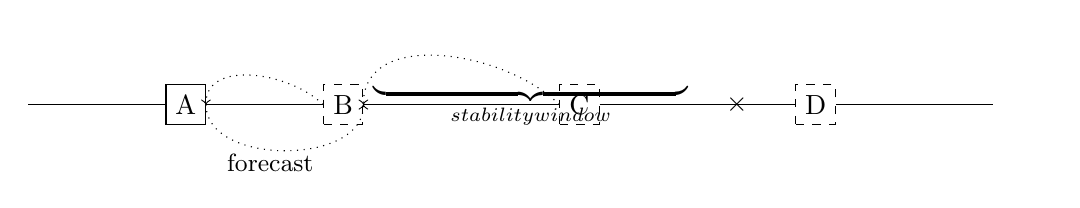
\begin{tikzpicture}
  [block/.style={rectangle,draw=black,minimum size=5mm}]
\path (-2,0) -- (11,0); % adjust bounding box
\node at (0,0) (A) [block] {A};
\node at (2,0) (B) [block, dashed] {B};
\node at (5,0) (C) [block, dashed] {C};
\node at (8,0) (D) [block, dashed] {D};
\draw (-2,0)   -- (A.west);
\draw (A.east) -- (B.west) node[pos=0.55,below=5mm]{\small forecast};
\draw (B.east) -- (C.west);
\draw (C.east) -- (D.west);
\draw (D.east) -- ++(2,0);
%
\draw [->, dotted] (B.west) to [out=135,in=90] (A.east);
\draw [->, dotted] (C.west) to [out=135,in=90] (B.east);
%
\draw [->, dotted] (A.east) to [out=270,in=270] (B.east);
\node at (B.east) [below=0.6, right] {$\underbrace{\hspace{4cm}}_\text{stability window}$};
\node at (7,0) {$\times$};
\end{tikzpicture}
\end{center}
%
We can use the ledger state after applying block $A$ (which we
have complete knowledge of) to validate any header up to the end of $B$'s
stability window: any changes that $A$ (or any block before $A$)
initiates we know about, and any changes that $B$ initiates cannot take effect
until that stability window ends. Therefore we can validate header $C$, but not
header $D$: block $B$ might have scheduled some changes to take effect at the
slot marked as $(\times)$ in the diagram, and we do not know what those effects
are.\footnote{It might be tempting to think that we can validate $D$ because if
we did have blocks $B$ and $C$, block $D$ would be evaluated against the ledger
state as it was after applying $C$, which is still within $B$'s stability
window. However, the slot number of $D$ (its location on the $x$-axis in the
diagram) matters, because changes are scheduled for slots.}

In chain sync we do not currently take advantage of the knowledge of the
location of header $B$.\footnote{\label{footnote:anchor-after-first-header}We
should change this. By anchoring the stability window at the last known block,
we only have a guarantee that we can validate $k$ headers, but we should really
be able to validate $k + 1$ headers in order to get a chain that is longer than
our own (\cref{low-density:tension}). If we anchored the stability window after
the first unknown header, where it \emph{should} be anchored, we can validate
$k$ headers \emph{after} the first unknown header, and hence $k + 1$ in total.
Concretely, we would have to extend the \lstinline!LedgerSupportsProtocol! class
with a function that forecasts the ledger view given a \emph{ticked} ledger
state. Taking advantage of this would then just be a minor additional
complication in the chain sync client.}  This means we have to be conservative:
all we know is that there could be \emph{some} block in between $A$ and $C$ that
might schedule some changes that are relevant for validating header $C$. In this
case we therefore assume that the stability window extends from $A$ instead:
%
\begin{center}
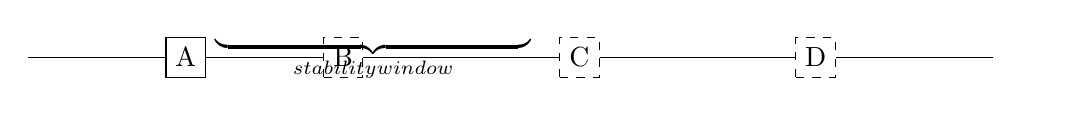
\begin{tikzpicture}
  [block/.style={rectangle,draw=black,minimum size=5mm}]
\path (-2,0) -- (11,0); % adjust bounding box
\node at (0,0) (A) [block] {A};
\node at (2,0) (B) [block, dashed] {B};
\node at (5,0) (C) [block, dashed] {C};
\node at (8,0) (D) [block, dashed] {D};
\draw (-2,0)   -- (A.west);
\draw (A.east) -- (B.west);
\draw (B.east) -- (C.west);
\draw (C.east) -- (D.west);
\draw (D.east) -- ++(2,0);
%
\node at (A.east) [below=0.6, right] {$\underbrace{\hspace{4cm}}_\text{stability window}$};
\end{tikzpicture}
\end{center}
%
In this example, that means we can validate $B$, but not $C$ (nor
$D$).\footnote{We could in principle shift this up by 1 slot: after all, the
very first next block after $A$ cannot be in the same slot as $A$. While EBBs
are an exception to that rule (\cref{ebbs}), we do not need to validate EBBs so
this is a rare example where EBBs do not cause a problem.}

\subsection{Tension with chain selection}
\label{low-density:tension}

Changes that affect the ledger view are scheduled for slots (often
for epoch boundaries, which happen at particular slots); the stability window
must therefore be defined in terms of slots as well. This means that
the number of \emph{headers} we can validate within a given stability window
depends on the density of that chain; if the chain we considered at the end
of the previous section looks like this instead
%
\begin{center}
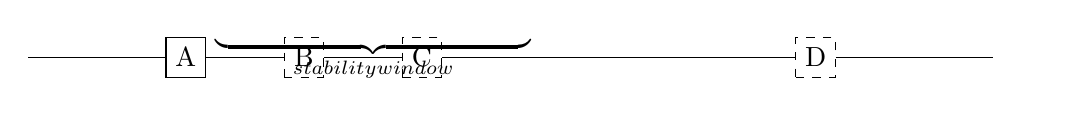
\begin{tikzpicture}
  [block/.style={rectangle,draw=black,minimum size=5mm}]
\path (-2,0) -- (11,0); % adjust bounding box
\node at (0,0) (A) [block] {A};
\node at (1.5,0) (B) [block, dashed] {B};
\node at (3,0) (C) [block, dashed] {C};
\node at (8,0) (D) [block, dashed] {D};
\draw (-2,0)   -- (A.west);
\draw (A.east) -- (B.west);
\draw (B.east) -- (C.west);
\draw (C.east) -- (D.west);
\draw (D.east) -- ++(2,0);
%
\node at (A.east) [below=0.6, right] {$\underbrace{\hspace{4cm}}_\text{stability window}$};
\end{tikzpicture}
\end{center}
%
we can validate headers $B$ and $C$ (but still not $D$).

There is a fundamental tension between the stability window defined in
\emph{slots}, and chain selection preferring  longer chains: chains that have
more \emph{blocks}. In order to be able to do a meaningful comparison between
our chain and the candidate chain, we must be able to verify enough of that
candidate chain that the length of that verified prefix exceeds the length of
our own chain. Since the maximum rollback we support is $k$
(\cref{consensus:overview:k}), that means we must be able to validate at least
$k + 1$ headers. The tension is resolved by a theoretical result that says that
within $3k/f$ slots we \emph{will} see more than $k$ blocks (more precisely, the
probability that we see fewer than $k$ blocks in $3k/f$ slots is negligibly
small; \cite{cryptoeprint:2017:573}). This therefore provides us with a suitable
choice for a stability window.

Unfortunately, while in theory there is no difference between theory and
practice, there is in practice. Currently, when all nodes in the system are
unable to produce blocks for an extended period of time, the system grinds to a
halt. Even if the underlying problem is resolved, nodes will refuse to create a
block if the distance between that block and the previous block exceeds the
stability window; after all, if they did produce a block, other nodes would be
unable to validate it. The former is easily resolved, this is merely a check in
the block production code; resolving the second problem is the topic of this
chapter.

It would be preferable to avoid the tension altogether, and schedule
changes that affect the ledger view for particular \emph{blocks} instead
(and consequently, have epoch boundaries also happen at certain blocks). This
however requires backing from theoretical research; we will come back to this
in \cref{future:block-vs-slot}.

\pagebreak

\subsection{Single-gap case}

It is tempting to think that when there is only a \emph{single} large gap
on the chain, there is no problem:
%
\begin{center}
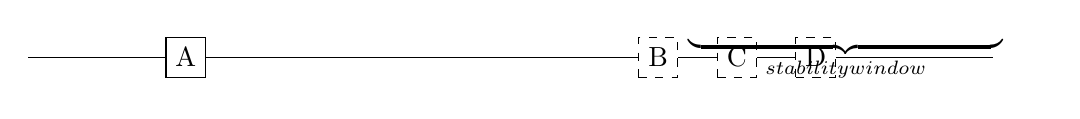
\begin{tikzpicture}
  [block/.style={rectangle,draw=black,minimum size=5mm}]
\path (-2,0) -- (11,0); % adjust bounding box
\node at (0,0) (A) [block] {A};
\node at (6,0) (B) [block, dashed] {B};
\node at (7,0) (C) [block, dashed] {C};
\node at (8,0) (D) [block, dashed] {D};
\draw (-2,0)   -- (A.west);
\draw (A.east) -- (B.west);
\draw (B.east) -- (C.west);
\draw (C.east) -- (D.west);
\draw (D.east) -- ++(2,0);
%
\node at (B.east) [below=0.6, right] {$\underbrace{\hspace{4cm}}_\text{stability window}$};
\end{tikzpicture}
\end{center}
%
The gap between $A$ and $B$ exceeds the stability window, but this
should not matter: it's not the stability window after $A$ that
matters, but the stability window after $B$. This seems to be a useful special
case: if a problem \emph{does} arise that prevents nodes from producing blocks
for an extended period of time, one might hope that this problem does not
immediately arise again after the nodes resume producing blocks.

As we saw, the consensus layer always conservatively anchors the stability
window at the last known block rather than the first header after the tip. We
could change this (and probably should; see
\cref{footnote:anchor-after-first-header}), but it turns out this does not
actually help very much for this particular problem. To see this, suppose there
is another node in the system which is currently on a fork that intersects with
this chain after some block $I$ before the gap:
%
\begin{center}
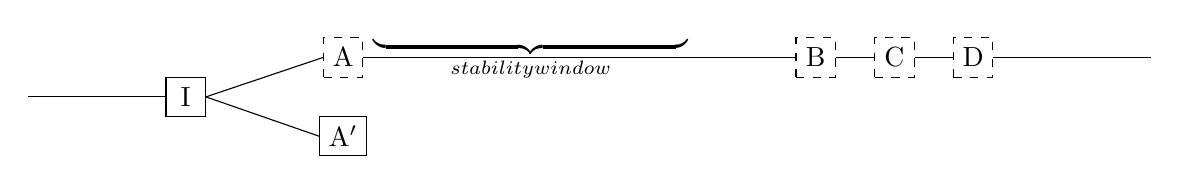
\begin{tikzpicture}[yscale=0.5,block/.style={rectangle,draw=black,minimum size=5mm}]
\node at (-2,-1) (I) [block] {I};
\node at (0,0) (A) [block, dashed] {A};
\node at (6,0) (B) [block, dashed] {B};
\node at (7,0) (C) [block, dashed] {C};
\node at (8,0) (D) [block, dashed] {D};
\draw (-4,-1)   -- (I.west);
\draw (I.east) -- (A.west);
\draw (A.east) -- (B.west);
\draw (B.east) -- (C.west);
\draw (C.east) -- (D.west);
\draw (D.east) -- ++(2,0);
%
\node at (A.east) [below=0.6, right] {$\underbrace{\hspace{4cm}}_\text{stability window}$};
%
\node at (0, -2) (A') [block] {A$'$};
\draw (I.east) -- (A'.west);
\end{tikzpicture}
\end{center}
%
The second node must execute a rollback to $I$ in order to be able to adopt
the new chain, but from \emph{its} perspective the first unknown block is $A$,
not $B$: hence the stability window \emph{must} be anchored at $A$, and the
node will be unable to bridge the gap.

\section{Pre-genesis}
\label{low-density:pre-genesis}

In this section we will consider how we might allow nodes to recover from a low
density chain, prior to the implementation of the genesis rule. An obvious
solution suggests itself: we could just allow chain sync to download blocks
when it needs to validate a header which is beyond its forecast range.

\subsection{Damage mitigation}

The reason the chain sync client doesn't normally download blocks is to limit
the amount of unnecessary work an attacker can make it do (prevent DoS attacks,
\cref{nonfunctional:network:headerbody}). We might therefore consider if we can
restrict \emph{when} we allow the chain sync client to download blocks. Ideally
we would do this only ``when necessary'': to bridge the gap on the honest chain.
Unfortunately, it is difficult to come up with a criterion that
approximates this ideal. Consider how the situation evolves from the point of
view of a single node:

\begin{center}
\begin{tikzpicture}[yscale=0.25]
%
\path (0, 0) coordinate(imm1) node{$\bullet$} node[above]{imm};
\draw (imm1) -- ++(-1,0);
\draw (imm1) -- ++(0.5,0);
\path (imm1) -- ++(0.5,0) -- ++(1,0) node[pos=0.5]{$\cdots$} -- ++(0.5,0) coordinate(cp1);
\draw (cp1) -- ++(-0.5,0);
\draw (cp1) -- ++(1, 1.5) -- ++(1,   0) node{$\bullet$};
\draw (cp1) -- ++(1, 0.5) -- ++(1.5, 0) node{$\bullet$};
\draw (cp1) -- ++(1,-0.5) -- ++(0.5, 0) node{$\bullet$};
\draw (cp1) -- ++(1,-1.5) -- ++(1,   0) node{$\bullet$};
\draw [very thick] (4.5,-2) -- (4.5,2) node[above]{now};
%
\path (0, -7) coordinate(imm2) node{$\bullet$} node[above]{imm};
\draw (imm2) -- ++(-1,0);
\draw (imm2) -- ++(0.5,0);
\path (imm2) -- ++(0.5,0) -- ++(1,0) node[pos=0.5]{$\cdots$} -- ++(0.5,0) coordinate(cp2);
\draw (cp2) -- ++(-0.5,0);
\draw (cp2) -- ++(1, 1.5) -- ++(1,   0) node{$\bullet$};
\draw (cp2) -- ++(1, 0.5) -- ++(1.5, 0) node{$\bullet$};
\draw (cp2) -- ++(1,-0.5) -- ++(0.5, 0) node{$\bullet$};
\draw (cp2) -- ++(1,-1.5) -- ++(1,   0) node{$\bullet$};
\draw [very thick] (5.5,-9) -- (5.5,-5) node[above]{now};
%
\path (0, -14) coordinate(imm3) node{$\bullet$} node[above]{imm};
\draw (imm3) -- ++(-1,0);
\draw (imm3) -- ++(0.5,0);
\path (imm3) -- ++(0.5,0) -- ++(1,0) node[pos=0.5]{$\cdots$} -- ++(0.5,0) coordinate(cp3);
\draw (cp3) -- ++(-0.5,0);
\draw (cp3) -- ++(1, 1.5) -- ++(1,   0) node{$\bullet$};
\draw (cp3) -- ++(1, 0.5) -- ++(1.5, 0) node{$\bullet$};
\draw (cp3) -- ++(1,-0.5) -- ++(0.5, 0) node{$\bullet$};
\draw (cp3) -- ++(1,-1.5) -- ++(1,   0) node{$\bullet$};
\path (4.5,-12.5) -- (7.5,-12.5) node[pos=0.5,above=-0.1]{$\overbrace{\hspace{3cm}}^\text{$> s$ slots}$};
\draw [very thick] (7.5,-16) -- (7.5,-12) node[above]{now};
%
\path (0, -21) coordinate(imm4) node{$\bullet$} node[above]{imm};
\draw (imm4) -- ++(-1,0);
\draw (imm4) -- ++(0.5,0);
\path (imm4) -- ++(0.5,0) -- ++(1,0) node[pos=0.5]{$\cdots$} -- ++(0.5,0) coordinate(cp4);
\draw (cp4) -- ++(-0.5,0);
\draw (cp4) -- ++(1, 1.5) -- ++(1,   0) node{$\bullet$} coordinate(before1);
\draw (cp4) -- ++(1, 0.5) -- ++(1.5, 0) node{$\bullet$};
\draw (cp4) -- ++(1,-0.5) -- ++(0.5, 0) node{$\bullet$} coordinate(before2);
\draw (cp4) -- ++(1,-1.5) -- ++(1,   0) node{$\bullet$};
\path (4.5,-19.5) -- (7.5,-19.5) node[pos=0.5,above=-0.1]{$\overbrace{\hspace{3cm}}^\text{$> s$ slots}$};
\draw [very thick] (10,-23) -- (10,-19) node[above]{now};
\path (before1) -- ++(5,0) coordinate(after1);
\path (before2) -- ++(6,0) coordinate(after2);
\draw (after1) node{$\bullet$} -- ++(2,0);
\draw (after2) node{$\bullet$} -- ++(2,0);
\end{tikzpicture}
\end{center}

\pagebreak

The node is tracking the chains of a number of upstream peers. These chains will
share some common prefix, which must at least include the tip of our own
immutable database (that is, the block $k$ blocks away from our tip), marked
``imm''. When block production is halted due to some problem, the gap between
the tips of the chains and the wallclock will start to increase; at some point
this gap will exceed the stability window. Finally, when the problem is resolved
the nodes will start producing blocks again.

\begin{assumption}
\label{never-only-malicious}
In the period where the honest nodes cannot produce any blocks, malicious nodes
cannot either. If that is not the case, we are in trouble anyway; that is a
problem which is well outside the scope of this chapter.
\end{assumption}

\Cref{never-only-malicious} seems to give some hope. We may not be able to
decide for any \emph{particular} chain if that chain happens to be the honest
chain. However, if \emph{none} of the chains contain any blocks in the gap, then
eventually it will be true for \emph{all} upstream peers that the gap from the
tip of that peer's chain to the wallclock exceeds the stability window. This
might suggest the following rule:

\begin{failedattempt}
Only allow the chain sync client to download blocks if this would be required
for \emph{all} peers.
\end{failedattempt}

Unfortunately, this rule does not work because as soon as we bridge the gap for
\emph{one} of our peers, that condition no longer holds:
%
\begin{center}
\begin{tikzpicture}[yscale=0.25]
\path (0, -21) coordinate(imm4) node{$\bullet$} node[above]{imm};
\draw (imm4) -- ++(-1,0);
\draw (imm4) -- ++(0.5,0);
\path (imm4) -- ++(0.5,0) -- ++(1,0) node[pos=0.5]{$\cdots$} -- ++(0.5,0) coordinate(cp4);
\draw (cp4) -- ++(-0.5,0);
\draw (cp4) -- ++(1, 1.5) -- ++(1,   0) node{$\bullet$} coordinate(before1);
\draw (cp4) -- ++(1, 0.5) -- ++(1.5, 0) node{$\bullet$};
\draw (cp4) -- ++(1,-0.5) -- ++(0.5, 0) node{$\bullet$} coordinate(before2);
\draw (cp4) -- ++(1,-1.5) -- ++(1,   0) node{$\bullet$};
\path (4.5,-19.5) -- (7.5,-19.5) node[pos=0.5,above=-0.1]{$\overbrace{\hspace{3cm}}^\text{$> s$ slots}$};
\draw [very thick] (10,-23) -- (10,-19) node[above]{now};
\path (before1) -- ++(5,0) coordinate(after1);
\draw (before2) -- ++(6,0) coordinate(after2);
\draw (after1) node{$\bullet$} -- ++(2,0);
\draw (after2) node{$\bullet$} -- ++(2,0);
\end{tikzpicture}
\end{center}
%
Now one of our chains has a tip which is near the wallclock, and so the
condition no longer holds. Okay, you might say, but it was true at \emph{some}
point, and when it was true, it would have allowed the chain sync client to
download blocks for \emph{any} peer. Thus, we could try the following rule:

\begin{failedattempt}
When we detect that the tips of all upstream peers are more than the stability
window away from the wallclock, give the chain sync client a chance to download
blocks for \emph{all} peers.
\end{failedattempt}

This \emph{might} work, but it's very stateful. What does ``all peers'' mean
exactly? All peers we are currently connected to? What if we connect to another
peer later? What if the node has restarted in the meantime, do we need to
persist this state? Will we need some notion of peer identity? Perhaps all of
these questions have answers, but this does not seem like a clean solution.

As a final attempt, we might try to ensure that there is only a \emph{single}
chain after we resolve the problem that was preventing block production.
Suppose this could somehow be guaranteed (out of band communication to agree on
a block in the common prefix, use a BFT-like leadership selection for a while,
etc.). Then we could try the following rule:

\begin{failedattempt}
When we detect that the tips of all upstream peers are more than the stability
window away from the wallclock, allow the chain sync client to download enough
blocks to bridge the gap for \emph{one} peer. Allow the other peers to bridge
the gap only if they contain the \emph{same} header after the gap.
\end{failedattempt}

Unfortunately, this still cannot work. Even if the honest nodes agree to only
produce a single chain after the gap, we cannot prevent an adversary from
constructing another chain. If the node then happens to pick the adversary's
chain as the one-and-only allowed header to jump the gap, it would be unable to
then switch to the honest chain later.

\pagebreak

\subsection{Damage analysis}

If we cannot limit when the chain sync client is allowed to download and
validate blocks, then let's analyse exactly what the possibility for denial of
service attacks really is.

\begin{lemma}
When the node is up to date, the chain sync client will never have to download
any blocks.
\end{lemma}

\begin{proof}
The Praos analysis \cite{cryptoeprint:2017:573} tells us that the honest chains
will not diverge by more than $k$ blocks, and that this means that their
intersection cannot be more than $3k/f$ slots away from the wallclock (provided
block production is not halted, of course). This means that any header that
would be more than the stability window away from the intersection point
would have a slot number past the wallclock, and would therefore be
invalid.\footnote{Though we allow for some minimal clock skew, headers past
the wallclock should be considered invalid if this exceeds $s$ slots from the
immutable tip, even if they would still fall within the permissible clock
skew. This is an edge case that was important for implementation of genesis
as well; see \cref{genesis:becoming-alert:DoS}.}
\end{proof}

This means that we only have to worry about DoS attacks while a node is syncing.
As a first observation, node performance is less critical here. The node is
anyway not producing blocks while syncing, so causing the node to slow down
temporarily is not a huge deal (\emph{cf.} also \cref{genesis:optimisations}
where we argue it's less essential during syncing to make the worst case
performance and the normal case performance the same).

It will therefore suffice to simply \emph{bound} the amount of work a malicious
node can make us do. We have to make sure that we can see at least $k+1$ headers
from each peer (we want to support a rollback of $k$ blocks, and chain selection
is based on length, so if we can validate $k+1$ headers, we have seen enough to
do a length comparison and decide we want to switch to the other chain). This
means we would need to download at most $k$ blocks.

This bounds the amount of \emph{memory} we might need to dedicate to any
chain,\footnote{Currently the length of the fragments we keep in memory for each
upstream peer is bound by the forecast range, but that natural bound would of
course no longer work if we allow the chain sync client to download blocks.} but
does not limit how much \emph{work} they can make us do: an attacker with even a
small amount of stake could construct lots of chains that fork off the main
chain, and so we'd end up downloading and validating lots of blocks. We can
limit the impact of this by rate limiting rollback messages, which would be
useful for other purposes as well.\footnote{For example, it can help avoid a DoS
attack where an attacker attempts to flood our volatile DB with lots of useless
blocks.}  Moreover, there is no real asymmetry here between the attacker and the
defender: the cost of downloading and validating a block on our side is  not too
dissimilar from the cost of producing and providing that block on the side of
the attacker, and all the attacker would gain in doing so is slow down a node's
syncing speed. (Admittedly, if we adopt more than $k$ blocks from the
adversarial chain we'd be in trouble, but that is a problem solved by the
Genesis chain selection rule).

\pagebreak

\section{Post-genesis}
\label{low-density:post-genesis}

With the implementation of the genesis rule, discussed in detail in
\cref{genesis}, some things get easier, but unfortunately some things get more
difficult.

\subsection{Pre-disaster genesis window}

Suppose the chain is operating as normal until disaster strikes and the nodes
stop producing blocks:
%
\begin{center}
\begin{tikzpicture}[yscale=0.5]
\draw
     (0,0)
  -- (3,0) node{$\bullet$} coordinate(i);
\draw (i) -- ++(1,  1) -- ++(1,   0);
\draw (i) -- ++(1,  0) -- ++(1.5, 0);
\draw (i) -- ++(1, -1) -- ++(0.5, 0);
\path
     (i)
  -- ++(2.5,  0) node[pos=0.5,above=0.5cm]{$\overbrace{\hspace{2.5cm}}^\text{$\le k$ blocks}$};
\draw [very thick] (6,-1.5) -- (6,2) node[above]{disaster};
\end{tikzpicture}
\end{center}
%
While the Genesis analysis \cite{cryptoeprint:2018:378} tells us that that
common intersection point is \emph{at most} $k$ blocks away, in practice it will
actually be much less than $k$ most of the time, a handful of blocks in typical
cases. This means that when the nodes start producing blocks again, chain
selection will be a looking at a window of $s$ slots where all chains have very
low density:\footnote{Prefix selection does a length comparison when we can see
all chains to their tip, meaning all chains terminate within the $s$ window. It
is important that we don't reinterpret that as ``all chains are less than $k$
\emph{blocks} away from the intersection point''. If we did, we would conclude
in this case that we can still do a length comparison when the chains continue
after the end of the disaster period; that is not correct: it would mean that
while the chains start are growing we would come to one conclusion, but then
once the chains grow past the window of $k$ blocks, we would switch to comparing
density and might come to a \emph{different} conclusion.}
%
\begin{center}
\begin{tikzpicture}[yscale=0.5]
\draw
     (0,0)
  -- (3,0) node{$\bullet$} coordinate(i);
\draw (i) -- ++(0.25,  1) -- ++(0.5,  0);
\draw (i) -- ++(0.25,  0) -- ++(0.75, 0);
\draw (i) -- ++(0.25, -1) -- ++(0.25, 0);
\draw [very thick] (4.5,-1.5) -- (4.5,2.5) node[above]{disaster\vphantom{y}};
\draw [very thick] (6.5,-1.5) -- (6.5,2.5) node[above]{recovery};
\draw [dashed]
     (i)
  -- ++( 0,  2)
  -- ++( 3,  0)
  -- ++( 0, -4)
  -- ++(-3,  0) node[pos=0.5,below]{$\underbrace{\hspace{3cm}}_\text{$s$ slots}$}
  -- cycle;
%
\draw (6.5,  1) -- (8.5,  1);
\draw (6.5,  0) -- (7.5,  0);
\draw (6.5, -1) -- (8,   -1);
\end{tikzpicture}
\end{center}
%
In effect we are doing a density comparison over very short fragments. In
general this is not meaningful; in the extreme case, where that fragment
contains only a single slot, density will either be 100\% or 0\%.
It is tempting to think that we could just \emph{grow} the genesis window to
include part of the post-disaster chain. Growing the genesis window is however
not sound: once we get more than $s$ slots away from the intersection point, an
adversary can start to influence the leadership schedule and so density
comparisons are no longer meaningful.

Essentially what this means is that after disaster recovery we arbitrarily pick
any of the chains from before the disaster to continue. This probably does not
matter too much; at worst more blocks are lost than strictly necessary, but
those transactions can be resubmitted and we're anyway talking about disaster
recovery; some loss is acceptable.\todo{Verify}

It might \emph{even} okay if the chain we happened to pick was constructed by an
adversarial node. After all, at most they can have constructed $k$ blocks, and
all they can do is selectively \emph{omit} transactions; if we continue the
chain based on such an adversarial chain, the damage they can do is very
limited.\todo{Verify}

\emph{However.} Suppose we do make an arbitrary choice and the chain resumes.
Nothing is preventing an adversary from forking off a new chain just prior to
the disaster region \emph{after the fact}. If they do, and new nodes joining
the system end up choosing that chain, they are in serious trouble; now they
are following a chain that is basically under the control of the adversary.

\pagebreak

This ability of adversaries to construct new forks before areas of low density
on the chain mean that these areas are a serious risk to security. Indeed,
somewhat ironically this risk is made \emph{worse} by the genesis rule. If we
look at chain length only, the honest chain will probably be longer than
whatever chain an attacker forges; but if we look at density, an attacker than
can even produce a single block in $s$ slots might already have a sufficient
advantage.

This means that some kind of disaster recovery becomes even more important
after we implement the genesis rule. Ideally we would patch the chain up,
but there is an easier option which can work (at least as a temporarily
solution): it suffices to hardcode a pre-disaster block as the agreed-on
pre-disaster tip.

\subsection{Post-disaster genesis window}

So far we've been talking about the genesis window as we approach the disaster.
Suppose we choose \emph{some} block as our pre-disaster tip; either by randomly
selecting one of the chains (or if by luck all chains happen to converge
pre-disaster) or by hardcoding a preference for a certain block:
%
\begin{center}
\begin{tikzpicture}[yscale=0.5]
\draw (0,0) -- (3,0) coordinate(i) node{$\bullet$};
\draw [dotted] (i) -- ++(0.25,  1) -- ++(0.5,  0);
\draw
     (i)
  -- ++(0.25,  0)
  -- ++(0.75, 0) node{$\bullet$} coordinate(pre-disaster-tip);
\draw [dotted] (i) -- ++(0.25, -1) -- ++(0.25, 0);
\draw [very thick] (4.5,-1.5) -- (4.5,2.5) node[above]{disaster\vphantom{y}};
\draw [very thick] (6.5,-1.5) -- (6.5,2.5) node[above]{recovery};
\draw [dashed]
     (pre-disaster-tip)
  -- ++( 0,  2)
  -- ++( 3,  0)
  -- ++( 0, -4)
  -- ++(-3,  0) node[pos=0.5,below]{$\underbrace{\hspace{3cm}}_\text{$s$ slots}$}
  -- cycle;
%
\draw (6.5,  1) -- (8.5,  1);
\draw (6.5,  0) -- (7.5,  0);
\draw (6.5, -1) -- (8,   -1);
\end{tikzpicture}
\end{center}
%
Having made this choice,  we are \emph{again} faced with a comparison between
chains which all have very low density within the window (in the extreme case,
even zero). This means that here we effectively have a \emph{second} arbitrary
choice between chains, with all the same dangers (in particular the danger of an
attacker forking off a new chain after the fact). However, in this case we have
a way out:
%
\begin{lemma}
\label{lemma:shift-genesis-window}
Suppose we have decided on a particular pre-disaster tip, and the chains we see
look like this:
%
\begin{center}
\begin{tikzpicture}[yscale=0.5]
\draw
     (0,0)
  -- (3,0) node{$\bullet$} node[above left]{tip} coordinate(tip);
\draw
     (tip)
  -- ++(4,1.5) node{$\bullet$}
  -- ++(2.5,0) node[right]{$\cdots$};
\draw
     (tip)
  -- ++(6,0.5) node{$\bullet$}
  -- ++(0.5,0) node[right]{$\cdots$};
\draw
     (tip)
  -- ++(5,-0.5) node{$\bullet$}
  -- ++(1.5,0) node[right]{$\cdots$};
\draw
     (tip)
  -- ++(3,-1.5) node{$\bullet$}
  -- ++(3.5,0) node[right]{$\cdots$};
%
\draw [dashed]
     (tip)
  -- ++(0,2)
  -- ++(4.5,0) node[pos=0.5, above]{$\overbrace{\hspace{4.5cm}}^\text{$s$ slots}$}
  -- ++(0,-4)
  -- ++(-4.5,0)
  -- cycle;
\end{tikzpicture}
\end{center}
%
Then we can shift up the genesis lookahead window until it starts at the
first block after the tip:
%
\begin{center}
\begin{tikzpicture}[yscale=0.5]
\draw
     (0,0)
  -- (3,0) node{$\bullet$} node[above left]{tip} coordinate(tip);
\draw
     (tip)
  -- ++(4,1.5) node{$\bullet$}
  -- ++(2.5,0) node[right]{$\cdots$};
\draw
     (tip)
  -- ++(6,0.5) node{$\bullet$}
  -- ++(0.5,0) node[right]{$\cdots$};
\draw
     (tip)
  -- ++(5,-0.5) node{$\bullet$}
  -- ++(1.5,0) node[right]{$\cdots$};
\draw
     (tip)
  -- ++(3,-1.5) node{$\bullet$}
  -- ++(3.5,0) node[right]{$\cdots$};
%
\draw [dashed]
     (tip) ++(3,0)
  -- ++(0,2)
  -- ++(4.5,0) node[pos=0.5, above]{$\overbrace{\hspace{4.5cm}}^\text{$s$ slots}$}
  -- ++(0,-4)
  -- ++(-4.5,0)
  -- cycle;
\end{tikzpicture}
\end{center}
\end{lemma}

\begin{proof}
The first block that could be produced by an adversary is the first block after
the tip. This adversarial block cannot influence the leadership schedule until
at least $3k/f$ slots later, which is also the size of the lookahead window
($s$). Therefore a density comparison within the shifted window will still
favour the honest chains.
\end{proof}
%
\Cref{lemma:shift-genesis-window} means that we can shift the genesis window
until after the disaster, and avoid the second arbitrary choice between chains.
In particular, it means we can definitely make it across the gap safely if we
\emph{mark} the before-disaster block (to avoid picking an adversary's block).

\pagebreak

\subsection{(No) need for gap jumping}

In \cref{low-density:pre-genesis} we discuss that prior to the implementation
of the genesis rule, we sometimes need to allow the chain sync client to
download blocks. Since chain selection was based on length, we need to be able
to validate a sufficient number of headers to get a fragment that is longer
than our current chain; in the case of a disaster, that might mean validating
a header that is more than $s$ slots away from our latest usable ledger state
to validate that header, and hence we may need to download some blocks.

The genesis rule, in principle, \emph{never needs to look past $s$ slots}.
It makes all of its decisions based on a window of $s$ slots; if a node reports
a header past the end of that window, that just tells us we have seen everything
we need to see about that chain within the window. There is no need to validate
this header: any headers \emph{within} the window contribute to the density
of the chain and are validated, any headers \emph{past} the window just cap
that density; nodes cannot increase their chain's density with an invalid
header past the window, and so nothing can go wrong if we do not validate that
header.

This changes however if we want to make use of \cref{lemma:shift-genesis-window}.
It is of course necessary that we validate the headers \emph{within} the window;
if we shift the window, we are no longer guaranteed that ``within the window''
is synonymous with ``at most $s$ slots away from the ledger state we have
available''.

Whether or not this opens us up to denial of service attacks depends
on when exactly we shift the window. However, if we do this only if we have some
kind of explicit disaster recovery (where we mark the pre-disaster block),
or if the density in the window we see drops below a certain threshold, then
the scope for a denial is service attack is very limited indeed.

\subsection{In the absence of adversaries}

In the consensus tests (\cref{testing:consensus}) periods where no blocks are
being produced are hard to avoid. However, we do not (currently) model
adversarial behaviour. This means that any kind of explicit disaster recovery is
not needed: if pre-disaster and post-disaster we end up picking an ``arbitrary''
chain, consensus is still guaranteed. After all, the choice is not ``arbitrary''
in the sense that different nodes may pick different chains; it is only
``arbitrary'' in the sense that we are doing a density comparison on a fragment
that is too short (it may be necessary to add a deterministic tie-breaker in
case there are multiple fragments with equal density).
